% -----------------------------------------------
% Template for SMC 2020
% adapted from previous SMC paper templates
% -----------------------------------------------

\documentclass[dvipsnames, pdftex]{article}
\usepackage{tikz}
% \tikzset{>=latex}
% \tikzstyle{block} = [draw,minimum size=0.5cm]
% \usetikzlibrary{math,arrows,positioning,shapes.geometric, decorations.markings}

\usepackage{smc2020}
\usepackage{times}
\usepackage{ifpdf}
\usepackage[english]{babel}
\usepackage{cite}
\usepackage{multirow}
\usepackage[]{algorithm2e, setspace}
%%%%%%%%%%%%%%%%%%%%%%%% Some useful packages %%%%%%%%%%%%%%%%%%%%%%%%%%%%%%%
%%%%%%%%%%%%%%%%%%%%%%%% See related documentation %%%%%%%%%%%%%%%%%%%%%%%%%%
\usepackage{amsmath} % popular packages from Am. Math. Soc. Please use the 
\usepackage{amssymb}
\usepackage{cases}
% related math environments (split, subequation, cases,
%\usepackage{amsfonts}% multline, etc.)
%\usepackage{bm}      % Bold Math package, defines the command \bf{}
%\usepackage{paralist}% extended list environments
%%subfig.sty is the modern replacement for subfigure.sty. However, subfig.sty 
%%requires and automatically loads caption.sty which overrides class handling 
%%of captions. To prevent this problem, preload caption.sty with caption=false 
%\usepackage[caption=false]{caption}
%\usepackage[font=footnotesize]{subfig}


%user defined variables
\def\papertitle{Real-time Implementation of a Physical Model of the Tromba Marina} %using Finite-Difference Schemes}
\def\firstauthor{Silvin Willemsen}
\def\secondauthor{Stefan Bilbao}
\def\thirdauthor{Michele Ducceschi}
\def\fourthauthor{Stefania Serafin}
% \def\firstauthor{Silvin Willemsen, Stefania Serafin}
% \def\secondauthor{Stefan Bilbao and Michele Ducceschi}

% adds the automatic
% Saves a lot of output space in PDF... after conversion with the distiller
% Delete if you cannot get PS fonts working on your system.

% pdf-tex settings: detect automatically if run by latex or pdflatex
\newif\ifpdf
\ifx\pdfoutput\relax
\else
   \ifcase\pdfoutput
      \pdffalse
   \else
      \pdftrue
\fi

\ifpdf % compiling with pdflatex
  \usepackage[pdftex,
    pdftitle={\papertitle},
    pdfauthor={\firstauthor, \secondauthor, \thirdauthor, \fourthauthor},
    bookmarksnumbered, % use section numbers with bookmarks
    pdfstartview=XYZ % start with zoom=100% instead of full screen; 
                     % especially useful if working with a big screen :-)
   ]{hyperref}
  %\pdfcompresslevel=9

  \usepackage{graphicx}
  % declare the path(s) where your graphic files are and their extensions so 
  %you won't have to specify these with every instance of \includegraphics
  \graphicspath{{./figures/}}
  \DeclareGraphicsExtensions{.pdf,.jpeg,.png}

  \usepackage[figure,table]{hypcap}

\else % compiling with latex
  \usepackage[dvips,
    bookmarksnumbered, % use section numbers with bookmarks
    pdfstartview=XYZ % start with zoom=100% instead of full screen
  ]{hyperref}  % hyperrefs are active in the pdf file after conversion

  \usepackage[dvips]{epsfig,graphicx}
  % declare the path(s) where your graphic files are and their extensions so 
  %you won't have to specify these with every instance of \includegraphics
  \graphicspath{{./figures/}}
  \DeclareGraphicsExtensions{.eps}

  \usepackage[figure,table]{hypcap}
\fi

%setup the hyperref package - make the links black without a surrounding frame
\hypersetup{
    colorlinks,%
    citecolor=black,%
    filecolor=black,%
    linkcolor=black,%
    urlcolor=black
}


% Title.
% ------
\title{\papertitle}

% Authors
% Please note that submissions are NOT anonymous, therefore 
% authors' names have to be VISIBLE in your manuscript. 
%
% Single address
% To use with only one author or several with the same address
% ---------------
%\oneauthor
%   {\firstauthor} {Affiliation1 \\ %
%     {\tt \href{mailto:author1@smcnetwork.org}{author1@smcnetwork.org}}}

%Two addresses
%--------------
\twoauthors
  {\firstauthor{ and }\fourthauthor} {Multisensory Experience Lab, CREATE \\ Aalborg University Copenhagen \\
    {\tt \href{mailto:sil@create.aau.dk}{\{sil, sts\}@create.aau.dk}}}
  {\secondauthor{ and }\thirdauthor} {Acoustics and Audio Group \\ University of Edinburgh \\ %
    {\tt {\{s.bilbao, michele.ducceschi\}@ed.ac.uk}}}

% Three addresses
% --------------
%  \threeauthors
%   {\firstauthor} {Affiliation1 \\ %
%      {\tt \href{mailto:author1@smcnetwork.org}{author1@smcnetwork.org}}}
%   {\secondauthor} {Affiliation2 \\ %
%      {\tt \href{mailto:author2@smcnetwork.org}{author2@smcnetwork.org}}}
%   {\thirdauthor} { Affiliation3 \\ %
%      {\tt \href{mailto:author3@smcnetwork.org}{author3@smcnetwork.org}}}
% \fourauthors
%   {\firstauthor} {Multisensory Experience Lab, CREATE \\ Aalborg University Copenhagen \\ %
%      {\tt \href{mailto:sil@create.aau.dk}{sil@create.aau.dk}}}
%   {\secondauthor} {Acoustics and Audio Group \\ University of Edinburgh \\ %
%      {\tt \href{mailto:s.bilbao@ed.ac.uk}{s.bilbao@ed.ac.uk}}}
%     {\thirdauthor} {Acoustics and Audio Group \\ University of Edinburgh \\ %
%      {\tt \href{mailto:michele.ducceschi@ed.ac.uk}{michele.ducceschi@ed.ac.uk}}}
%   {\fourthauthor} {Multisensory Experience Lab, CREATE \\ Aalborg University Copenhagen \\ %
%      {\tt \href{mailto:sts@create.aau.dk}{sts@create.aau.dk}}}

% ***************************************** the document starts here ***************
\usepackage{xcolor}
\def\SBcomment[#1]{\textcolor{Red}{#1}}
\def\SWcomment[#1]{\textcolor{Bittersweet}{#1}}
\def\MDcomment[#1]{\textcolor{Blue}{#1}}
\def\SScomment[#1]{\textcolor{OliveGreen}{#1}}

\begin{document}
%
\capstartfalse
\maketitle
\capstarttrue
%
\begin{abstract}
You can place comments in colour if you want :) Like \SBcomment[this (Stefan)], \MDcomment[this (Michele)] or \SScomment[this (Stefania)].
\end{abstract}
%

\section{Introduction}\label{sec:introduction}
\SScomment[Instead of starting by talking about PMs, I would talk about the tromba marina. I can take care of this.]

 
 
   \begin{figure}
  \centering
  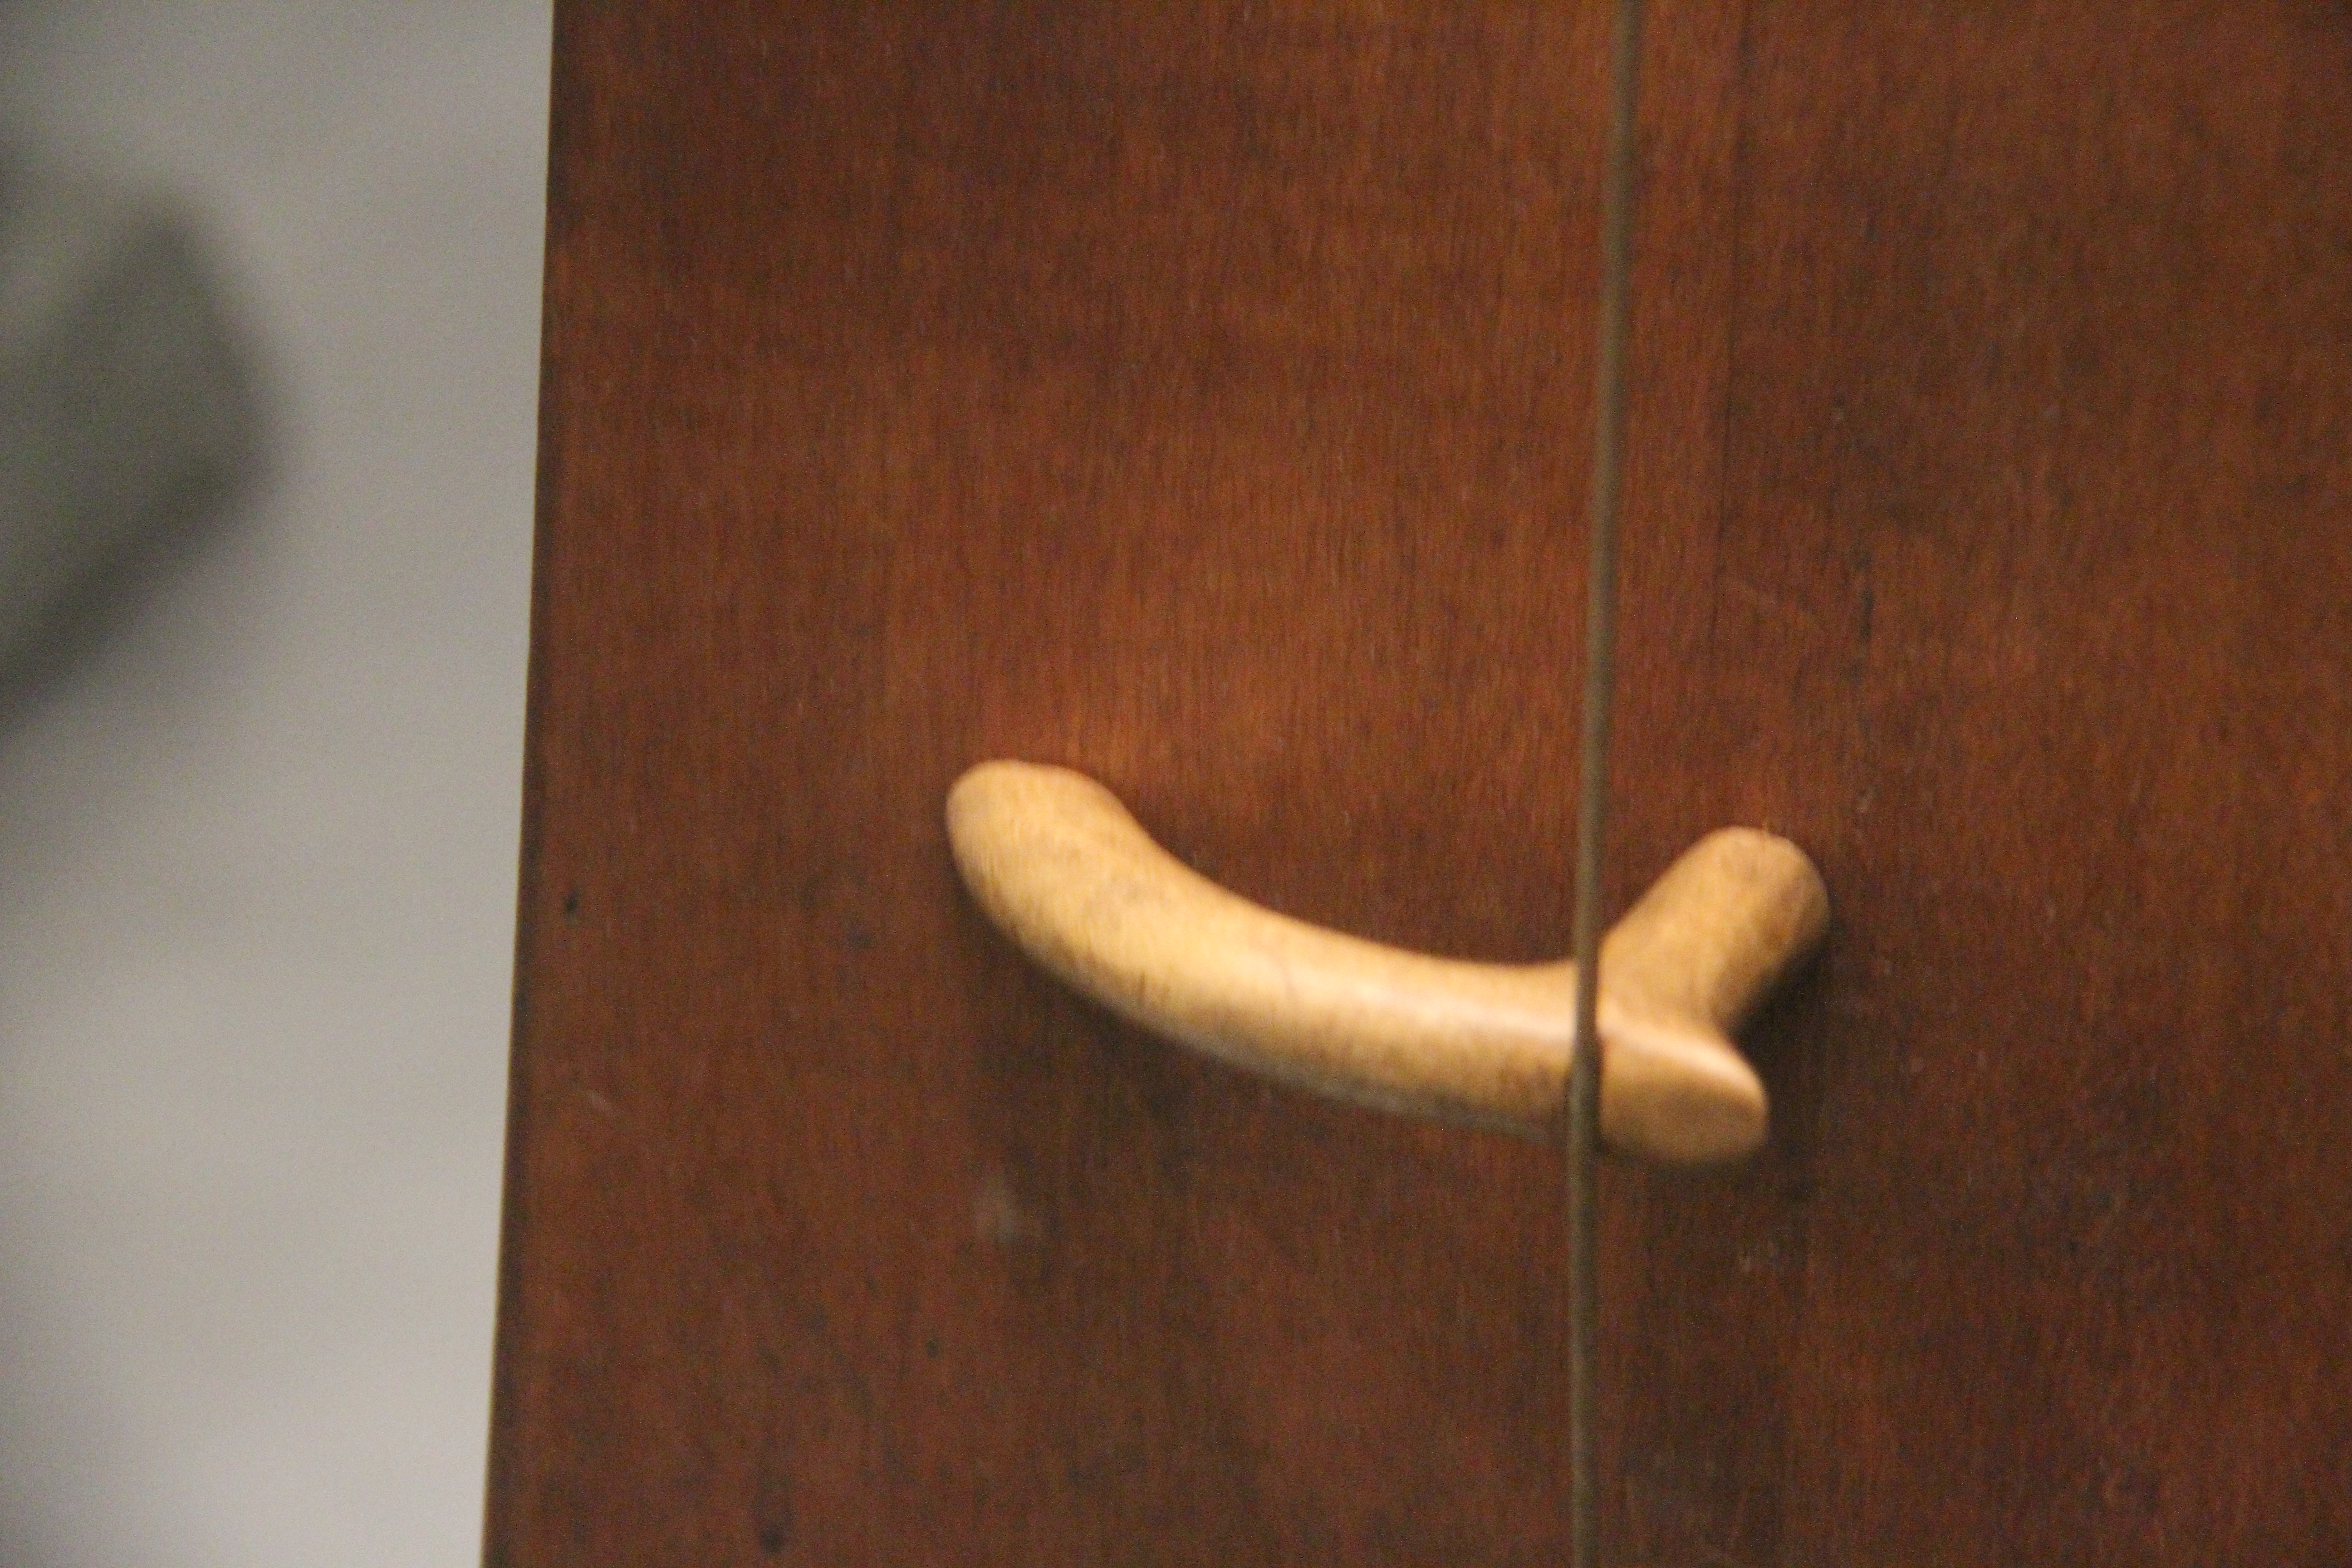
\includegraphics[width=\columnwidth]{IMG_7982.JPG}
  \caption{The bridge of the tromba marina from the Danish Music Museum in Copenhagen. }
  \label{fig:bridge}
\end{figure}

Simulating musical instruments using physical models has several purposes. One is the emulation of instruments that, due to fragility, rarity or value, are no longer in playing condition. In this paper, we present a real-time implementation of a physical model of the tromba marina, a tall bowed monochord from medieval Europe~\cite{encyclopaedia2020}. One string rests on a loose bridge that rattles against the body when the string is bowed. Interestingly, this creates a sound that has trumpet-like qualities, hence the name. 

Physical modelling for sound synthesis has a long history. Various techniques have been developed to simulate real-world instruments, including mass-spring systems~\cite{cadoz79, cadoz83, cadoz1993cordis}, digital waveguides~\cite{smith1992physical} and modal synthesis~\cite{morrison1993mosaic}. 
\SBcomment[can probably use just one of the Cadoz refs]

Finite-difference time-domain (FDTD) methods were first used for sound synthesis by Hiller and Ruiz in ~\cite{Ruiz1969, Hiller1971, Hiller2}, and later by Chaigne et al. in ~\cite{Chaigne92, Chaigne} and elaborated upon by Bilbao and colleagues in ~\cite{bilbao2009numerical, Bilbao2018:Tutorial}. Compared with other techniques, FDTD methods are more computationally expensive, but easily generalisable and flexible---no assumptions of linearity of travelling wave solutions are employed. Our goal is to implement these accurate techniques in real-time and thereby make the simulations playable for the users. 

The behaviour of musical instruments can be well described by partial-differential equations (PDEs). \textbf{$\leftarrow$ probably used exactly like this before}

\SBcomment[Probably don't need this paragraph above]

The emulation of nonlinear collision interactions in musical instruments normally requires the use of iterative solvers (such as, e.g. Newton-Raphson) \cite{Bilbao15}. For the non-linear collisions present in the instrument, a method recently proposed in the field of audio by Ducceschi and Bilbao in~\cite{Ducceschi2019} allows such iterative methods to be sidestepped. It is thus suited  to creating a real-time implementation of the tromba marina.

This paper is structured as follows: Section \ref{sec:models} presents the models used, Section \ref{sec:disc} shows 

\section{Models}\label{sec:models}
The tromba marina can be subdivided into three main components: the string, the bridge and the body. In this section, the PDEs of the different components in isolation will be given in the form
\begin{equation}\label{eq:PDEform}
    \mathcal{L}u = 0,
\end{equation}
with linear (partial) differential operator $\mathcal{L}$ and $u = u(\boldsymbol{x},t)$ describes the component state over time $t$ and space $\boldsymbol{x}\in\mathcal{D}$, where the dimensions of domain $\mathcal{D}$ depend on the component at hand. As different models share variable names, subscripts `$\text{s}$', `$\text{m}$' and `$\text{p}$' are added to denote that, among others, the variable $u$, domain ${\mathcal D}$ or operator ${\mathcal L}$ applies to the string, bridge (mass) or body (plate), respectively.

\subsection{Bowed Stiff string}
Consider a damped stiff string of length $L$ (m), with domain $\mathcal{D} = \mathcal{D}_\text{s} = [0,L]$ and state variable $u = u_\text{s}(x,t)$.  %\SBcomment[Too early here to introduce the differential operators...because you are talking about general linear operators here! They may not even be necessarily partial differential operators.] 
With reference to \eqref{eq:PDEform}, we define the operator $\mathcal{L} = \mathcal{L_\text{s}}$ as
\begin{equation}
    \mathcal{L}_\text{s} = \rho_\text{s} A \partial_t^2 - T\partial_x^2 + E_\text{s}I\partial_x^4+2\rho_\text{s} A\sigma_{0,\text{s}}\partial_t-2\rho_\text{s} A\sigma_{1,\text{s}}\partial_t\partial_x^2,
\end{equation}
Here, $\partial_{t}$ and $\partial_{x}$ indicate partial differentiation with respect to $t$ and $x$. The various parameters appear as: material density $\rho_\text{s}$ (kg$\cdot$m$^{-3}$), cross-sectional area $A = \pi r^2$ (m$^2$), radius $r$ (m), tension $T = (2f_{0,\text{s}}L)^2\rho_\text{s}A$ (N), fundamental frequency $f_{0,\text{s}}$ (s$^{-1}$), Young's modulus $E_\text{s}$ (Pa), moment of inertia $I=\pi r^4 / 4$ (m$^4$), and loss coefficients $\sigma_{0,\text{s}}$ (s$^{-1}$) and $\sigma_{1,\text{s}}$ (m$^2$/s). We set the boundary conditions to be simply supported so that
\begin{equation}\label{boundary}
    u_\text{s} = \partial_x^2u_\text{s} = 0, \quad \text{where} \quad x = 0, L.
\end{equation}
\SWcomment[In the DAFx paper from last year we wrote $x = 0, L$ instead of $x = {[}0, L{]}$, as -- in this case -- we don't want to specify a domain single locations instead. Which is correct?]
As the string is excited using a bow, Equation \eqref{eq:PDEform} may be augmented as:
\begin{equation}\label{eq:bowedString}
    \mathcal{L}_\text{s}u_\text{s} = -\delta(x-x_\text{b})F_\text{b}\Phi(v_\text{rel}),
\end{equation}
with externally supplied downward bow force $F_\text{b} = F_\text{b}(t)$ (N), spatial Dirac delta function $\delta(x-x_\text{b})$ selecting the bow position $x_\text{b} = x_\text{b}(t)\in \mathcal{D}_\text{s}$ (m), dimensionless friction characteristic
\begin{equation}
    \Phi(v_\text{rel}) = \sqrt{2a}v_\text{rel}e^{-av_\text{rel}^2+1/2},
\end{equation}
with free parameter $a$. The relative velocity between the string at bowing location $x_\text{b}$ and the externally supplied bow velocity $v_\text{b} = v_\text{b}(t)$ (m/s) is defined as:
\begin{equation}
    v_\text{rel} = \partial_tu_\text{s}(x_\text{b},t) - v_\text{b}.
\end{equation}

\subsection{Bridge}
The bridge is modelled as a simple mass with a linear restoring force. As this system is point-like, % or zero-dimensional, 
the state variable $u = u_\text{m}(t)$ and the definition of domain $\mathcal{D}$ is unnecessary. The operator $\mathcal{L}=\mathcal{L}_\text{m}$ is defined as
\begin{equation}
    \mathcal{L}_\text{m}=M\frac{d^2}{dt^2}+M\omega_0^2+MR\frac{d}{dt},
\end{equation}
\SWcomment[normal time derivative like this?] with mass $M$ (kg), linear angular frequency of oscillation $\omega_0=2\pi f_{0,\text{m}}$,  (s$^{-1}$), fundamental frequency $f_{0,\text{m}}$ (s$^{-1}$) and damping coefficient $R$ (s$^{-1}$).
\begin{figure}[ht]
    \centering
    \begin{tikzpicture}
    
    \def\radius{6}; % Radius of the string (>2!)
    \pgfmathsetmacro{\reps}{3}; % How may back-and-forths in the drawing of the springs
    \def\horShift{0.5}; %how far the bow is shifted to the right in b)
    \def\bowSpacing{0.2};
    \def\drawingSpacing{1.5}
    \def\bowWidth{5};
    
    \def\woodWidth{0.7}; %>0.3
    \def\bridgeHeight{3};
    \def\bridgeWidth{5};
    \def\cornerRadius{0.1};
    \def\stringWidth{0.15};
    \pgfmathsetmacro{\tinyRadius}{\stringWidth*0.1};
    \pgfmathsetmacro{\stringWidthMinTinyRad}{((\stringWidth-(2*\tinyRadius)))*0.5};
    %straight side
    \draw[-] (0, \bridgeHeight - \cornerRadius) -- (0, 0) node (line) {};
    \draw (0,0) arc(180:270:\cornerRadius cm and \cornerRadius cm);
    \draw (0,\bridgeHeight - \cornerRadius) arc(180:90:\cornerRadius cm and \cornerRadius cm);
    \draw[-] (\cornerRadius, -\cornerRadius) -- (\woodWidth - \cornerRadius, -\cornerRadius) node (line2) {};
    \draw (\woodWidth - \cornerRadius, -\cornerRadius) arc(270:360:\cornerRadius cm and \cornerRadius cm);
    \draw[-] (\woodWidth, 0) -- (\woodWidth, \bridgeHeight - \woodWidth - \cornerRadius) node (line) {};
    \draw (\woodWidth, \bridgeHeight - \woodWidth - \cornerRadius) arc(180:90:\cornerRadius cm and \cornerRadius cm);
    
    %%% string cavity %%%
    
    % define left and right position of the string cavity
    \pgfmathsetmacro{\leftStringPos}{\woodWidth * 0.5 - \stringWidth * 0.5};
    \pgfmathsetmacro{\rightStringPos}{(\woodWidth + \stringWidth) * 0.5};
    
    %line to cavity
    \draw[-] (\cornerRadius, \bridgeHeight) -- (\leftStringPos, \bridgeHeight) node (line) {};
   
    %tiny arc
    \draw (\leftStringPos, \bridgeHeight) arc(90:0:\tinyRadius cm and \tinyRadius cm);
    
    %stringarc
    \draw (\leftStringPos + \tinyRadius, \bridgeHeight - \tinyRadius) arc(180:360:\stringWidthMinTinyRad cm and \stringWidthMinTinyRad cm);
    %tinyarc
    \draw (\rightStringPos - \tinyRadius, \bridgeHeight - \tinyRadius) arc(180:90:\tinyRadius cm and \tinyRadius cm);
    
    % line to rest of bridge
    \draw[-] (\rightStringPos, \bridgeHeight) -- (\woodWidth + \cornerRadius, \bridgeHeight) node (line2) {};
    
    %bottom of arc
    
    \pgfmathparse{\bridgeHeight-\woodWidth};
    \draw (\woodWidth + \cornerRadius, \bridgeHeight - \woodWidth) arc(90:0:\bridgeWidth cm and \pgfmathresult cm);
    
    %% bottom of rattle
    
    %cur x-pos
    \pgfmathparse{\woodWidth + \bridgeWidth + \cornerRadius};
    \draw (\pgfmathresult, 0) arc(180:270:\cornerRadius cm and \cornerRadius cm);
    \draw[-] (\pgfmathresult + \cornerRadius, -\cornerRadius) -- ({\woodWidth + \bridgeWidth + \woodWidth}, -\cornerRadius) node (line) {};
    \pgfmathparse{2.0 * \woodWidth + \bridgeWidth};
    \draw (\pgfmathresult, -\cornerRadius) arc(270:360:\cornerRadius cm and \cornerRadius cm);
    
    %% top part of the arc
    \pgfmathsetmacro{\toparc}{\bridgeWidth + \woodWidth};
    \pgfmathparse{\bridgeWidth + 2.0*\woodWidth + \cornerRadius};
    \draw (\pgfmathresult, 0) arc(0:90:\toparc cm and \bridgeHeight cm);
    
    
    
    %%%% Annotations %%%%
    \def\arrowLength{0.5};
    \draw[<-] (\woodWidth + 0.1, 0) -- (\woodWidth + 0.1 + \arrowLength, 0) node [right] (TextNode) {a)};
    \draw[<-] (\woodWidth + \cornerRadius + \bridgeWidth - 0.1 , 0) -- (\woodWidth + \cornerRadius + \bridgeWidth - 0.1 - \arrowLength, 0) node [left] (TextNode) {b)};
    \draw[<-] (\woodWidth * 0.5, \bridgeHeight + 0.05) |- (\woodWidth, \bridgeHeight + 0.25) node [right] (TextNode) {c)};
    \end{tikzpicture}
    \caption{Diagram of the bridge (view from bottom of the tromba marina). Indicated are: a) the pivoting point always in contact with the body, b) the rattling point colliding with the body, and c) the string cavity straight above the middle of the pivoting point.}
    \label{fig:bridge}
\end{figure}

\subsection{Body}
The body is simplified to a two-dimensional plate with side-lengths $L_x$ and $L_y$, domain $\mathcal{D} = \mathcal{D}_\text{p} = [0,L_x] \times [0,L_y]$ and state variable $u = u_\text{p}(x,y,t)$. Using the 2D Laplacian
\begin{equation}
    \Delta \triangleq \partial_x^2+\partial_y^2,
\end{equation}
the operator $\mathcal{L} = \mathcal{L}_\text{p}$ can be defined as
\begin{equation}
    \mathcal{L}_\text{p} = \rho_\text{p}H\partial_t^2 + D\Delta\Delta +2\rho_\text{p}H\sigma_{0,\text{p}}\partial_t-2\rho_\text{p}H\sigma_{1,\text{p}}\partial_t\Delta,
\end{equation}
with material density $\rho_\text{p}$ (kg$\cdot$m$^{-3}$), plate thickness $H$ (m), stiffness coefficient $D = E_\text{p}H^3/12(1-\nu^2)$, Young's modulus $E_\text{p}$ (Pa), dimensionless Poisson's ratio $\nu$, and loss coefficients $\sigma_{0,\text{p}}$ (s$^{-1}$) and $\sigma_{1,\text{p}}$ (m$^2$/s). The boundary conditions of the plate are set to be clamped so that
\begin{equation}
    u_\text{p} = {\bf n} \cdot \nabla u_\text{p} = 0.
\end{equation}
where $\nabla u_\text{p}$ is the gradient of $u_\text{p}$, and where ${\bf n}$ indicates a normal to the plate boundary.
\subsection{Collisions}
It can be argued that the greatest contributor to the characteristic sound of the tromba marina is the rattling bridge colliding with the body. A collision can be modelled by including a term to the PDEs described above describing the potential energy of the system (further referred to as \textit{the potential}) \cite{Ducceschi2019}. For the bridge-body interaction this potential is defined as follows
\begin{equation}\label{eq:potential}
    \phi_\text{mp}(\eta_\text{mp}, t) = \frac{K_\text{mp}}{\alpha_\text{mp}+1}[\eta_\text{mp}]_+^{\alpha_\text{mp}+1}, \ K_\text{mp} \geq 0,\ \alpha_\text{mp} \geq 1,
\end{equation}
where $K_\text{mp}$ is the collision stiffness (N/m), $\alpha_\text{mp}$ is the non-linear collision coefficient \textbf{check units here..}, and $\eta_\text{mp} = \eta_\text{mp}(t)$ is the distance between the rattling part of the bridge and the body at the point of collision (m). Furthermore, and $[\eta_\text{mp}]_+ = 0.5(\eta_\text{mp}+|\eta_\text{mp}|)$ is the positive part of $\eta_\text{mp}$. The term which can then be included in the PDEs is $\phi_\text{mp}' = d\phi_\text{mp}/d\eta_\text{mp}$. As described in \cite{Falaize2016a:SMC2020, Falaize2016b:SMC2020, Lopes:SMC2020, Ducceschi2019}, using this form of the potential requires using iterative methods for solving its discrete counterpart. The authors proposed to rewrite the potential to
\begin{equation}
    \psi = \sqrt{2\phi},
\end{equation}
and the term included in the PDEs to
\begin{equation}\label{eq:phiToPsi}
    \phi' = \psi\psi' = \psi\frac{d\psi}{d\eta}\  \xrightarrow{\text{chain rule}}\ \psi\frac{\dot \psi}{\dot \eta}
\end{equation}
where the dot operator denotes a derivative with respect to time. Equation \eqref{eq:phiToPsi}, as can be seen in Section \ref{sec:disc}, can be explicitly calculated. 

As the string rests on the bridge, the interaction between these components needs to be modelled as well. Even though the bridge-body interaction is perpendicular to the string-bridge interaction, we can model them as being parallel, assuming that a ``horizontal" movement of the string causes a ``vertical movement" of the rattling part of the bridge. We can use an alternative version of the potential in Equation~\eqref{eq:potential} described in \cite{Bilbao2019} to make the collision two-sided acting as a connection:
\begin{equation}\label{eq:phiConnection}
    \phi_\text{sm}(\eta_\text{sm}, t) = \frac{K_\text{sm}}{\alpha_\text{sm}+1}|\eta_\text{sm}|^{\alpha_\text{sm}+1},
\end{equation}
%
where $\eta_\text{sm} = \eta_\text{sm}(t)$ is the distance between the string at the location of the bridge and the bridge itself. Including the effect of the bow from Equation \eqref{eq:bowedString}, Equation \eqref{eq:PDEform} for all components can be rewritten to get the complete system:
\begin{subnumcases}{\label{eq:fullSystem}}
% \begin{aligned}
    \mathcal{L}_\text{s}u_\text{s} &$=-\delta(x-x_\text{b})F_\text{b}\Phi(v_\text{rel})$ \label{eq:stringPotential}\\
    & $\quad\ \,\!\!+\  \delta(x-x_\text{sm})\psi_\text{sm}\psi_\text{sm}'$\nonumber\\
    \mathcal{L}_\text{m}u_\text{m} &$= -\psi_\text{sm}\psi_\text{sm}' + \psi_\text{mp}\psi_\text{mp}',$\label{eq:massPotential}\\
    \mathcal{L}_\text{p}u_\text{p} &$= -\delta(x-x_\text{mp}, y-y_\text{mp})\psi_\text{mp}\psi_\text{mp}',$\qquad\label{eq:platePotential}\\
    \eta_\text{sm} &$= u_\text{m} - u_\text{s}(x_\text{sm}, t),$\\
    \eta_\text{mp} &$=  u_\text{p}(x_\text{mp}, y_\text{mp}, t) - u_\text{m},$
% \end{aligned}
\end{subnumcases}
where $x_\text{sm} \in \mathcal{D}_\text{s}$ is the location of the bridge along the string and $(x_\text{mp}, y_\text{mp}) \in \mathcal{D}_\text{p}$ is where the bridge collides with the body.
\SBcomment[15a seems incorrect---you need a separate Dirac in order to emulate the string/mass connection, which is pointwise. Above it looks like it is distributed. Similarly for 15c, and here you will need a separate 2D Dirac definition (you can use $\delta^{(2)}$ for this). ] \SWcomment[how would I use $\delta^{(2)}$ in this situation? I now wrote it out like I did for the string.]
Note that the potentials belonging to a single collision 
in the above system have inverse signs as the collision force acts inversely on the two components. \textbf{not sure if this sentence is necessary, and otherwise rewrite..}
\section{Discretisation}\label{sec:disc}
The system found in the Equations in \eqref{eq:fullSystem} is discretised using FDTD methods. These methods subdivide the continuous system in grid points in space and samples in time. To approximate the state of a system in isolation we use
\begin{equation}\label{eq:generalDisc}
    u(\boldsymbol{x},t) \approx u^n_{\boldsymbol{l}}, 
\end{equation} 
where grid function $u^n_{\boldsymbol{l}}$ is a discrete version of $u({\boldsymbol{x}},t)$ sampled at $t=nk$ with time step $k$ (s), sample $n \in \mathbb{N}$ and location $\boldsymbol{l}$ that depends on domain $\mathcal{D}$ of the system at hand. In the case of the string, we use $x=lh_\text{s}$ with grid spacing $h_\text{s}$ (m), $\boldsymbol{l} = l \in [0,\hdots, N-1]$ and total number of grid points $N=L/h_\text{s}$ to yield $u_\text{s}(x,t) \approx u_{l,\text{s}}^n$. 

As the bridge is point-like, a definition of $\boldsymbol{l}$ is unnecessary and $u_\text{m}(t) \approx u_\text{m}^n$. 

In the case of the body, we use $x=lh_\text{p}$ and $y=mh_\text{p}$ to get $u_\text{p}(x, y, t) \approx u_{(l,m),\text{p}}^n$ where $\boldsymbol{l} = (l,m)$ with $l\in[0,\hdots,N_x-1]$ and $m\in[0,\hdots,N_y-1]$. Here, $N_x = L_x / h_\text{p}$ and $N_y = L_y / h_\text{p}$ are the horizontal and vertical number of points respectively.

%  = \boldsymbol{l}h$ with grid spacing $h$ and $\boldsymbol{l}$ describes the coordinates of the points in an isolated system (string, mass or plate) and
 
The discretisation of and expansion of operator $\mathcal{L}\approx \ell$ in the case of stiff strings, mass-spring systems and plates using FDTD methods are well covered in the literature \cite{Bilbao2009:NumericalSoundSynthesis}. To obtain the highest accuracy possible while keeping the system explicit (except for the bow), centered differences have been chosen where possible (see Equation \eqref{eq:discTimeOperators}). 

Grid spacings $h$ are calculated using, in the case of the stiff string,
\begin{equation}
    h_\text{s} = \sqrt{\frac{c^2k^2+4\sigma_1k+\sqrt{(c^2k^2+4\sigma_1k)^2+16\kappa^2k^2}}{2}},
\end{equation}
and in the case of the plate,
\begin{equation}
    h_\text{p} = 2\sqrt{k\left(\sigma_1 + \sqrt{\kappa^2 + \sigma_1^2}\right)}\ .
\end{equation}
\subsection{Collisions using non-iterative methods}
Before going into discretising the collision and connection terms in the system described in \eqref{eq:fullSystem}, some finite difference operators are introduced.
\subsubsection{Operators}
The identity and temporal shift operators are defined as
\begin{equation}
    1\eta^n = \eta^n, \quad e_{t+}\eta^n = \eta^{n+1}, \quad e_{t-}\eta^n = \eta^{n-1}.
\end{equation}
% similarly for interleaved grid points
% \begin{equation}
%     e_{t+}\psi^{n-1/2} = \psi^{n+1/2}, \quad e_{t-}\psi^{n+1/2} = \psi^{n-1/2}.
% \end{equation}
Using these, the operators for the forward, backward and centered time differences can be defined as
\begin{equation}\label{eq:discTimeOperators}
    \delta_{t+} = \frac{e_{t+} - 1}{k},\ \delta_{t-} = \frac{1 - e_{t-}}{k},\ \delta_{t\cdot} = \frac{e_{t+}-e_{t-}}{2k},
\end{equation}
and are all approximations to a first-order time derivative. Furthermore, forwards and backwards averaging operators are defined as
\begin{equation}
    \mu_{t+} = \frac{e_{t+} + 1}{2}, \quad \mu_{t-} = \frac{1 + e_{t-}}{2}.
\end{equation}
and can be used to describe interleaved grid points $n+1/2$ and $n-1/2$.
\subsubsection{Explicit collisions}
For the discrete-time definition of the collision terms in \eqref{eq:fullSystem} we can use 
\begin{equation}
    \psi\approx \mu_{t+}\psi^{n-1/2}\quad \text{and} \quad \psi' \approx \frac{\delta_{t+}\psi^{n-1/2}}{\delta_{t\cdot}\eta^n},
\end{equation}
% \begin{equation}
%     g^n = \frac{\delta_{t+}\psi^{n-1/2}}{\delta_{t\cdot}\eta^n},
% \end{equation}
where $\psi$ at interleaved grid point $n-1/2$ is defined as
\begin{equation}
    \psi^{n-1/2} = \mu_{t-}\psi^n.
\end{equation}
For a system that has a single (upward) collision we get
\begin{equation}\label{eq:dummySystem}
    \ell u^n_{\boldsymbol{l}} = J(\boldsymbol{x}_\text{c})\left(\mu_{t+}\psi^{n-1/2}\right)\frac{\delta_{t+}\psi^{n-1/2}}{\delta_{t\cdot}\eta^n},
\end{equation}
where $J(\boldsymbol{x}_\text{c})$ is a spreading operator applying the collision force to coordinate $\boldsymbol{x}_\text{c}$, which, in the simplest case, is defined as \cite{bilbao2009numerical}
\begin{equation}
   J(\boldsymbol{x}_\text{c}) = \begin{cases}
       \frac{1}{h^d}, & \boldsymbol{l} = \boldsymbol{l}_\text{c} = \text{round}(\boldsymbol{x}_\text{c} / h)\\
       0, & \text{otherwise}.
   \end{cases}
\end{equation}
Here, $d$ is the number of dimensions of domain $\mathcal{D}$ that $\boldsymbol{x}$ is defined for, i.e., $d=0$ for the bridge, $d=1$ for the string, and $d=2$ for the plate.

To continue, we use the identity 
\begin{equation}\label{eq:identity}
    \mu_{t+}\psi^{n-1/2} = \frac{k}{2}\delta_{t+}\psi^{n-1/2}-\psi^{n-1/2}
\end{equation}
and define
\begin{equation}\label{eq:gn}
    %\psi' \approx 
    g^n = \frac{\delta_{t+}\psi^{n-1/2}}{\delta_{t\cdot}\eta^n}
\end{equation}
which can be rewritten to
\begin{equation}\label{eq:gnRewritten}
    \delta_{t+}\psi^{n-1/2} = g^n\delta_{t\cdot}\eta^n.
\end{equation}
Then, inserting \eqref{eq:gnRewritten} into \eqref{eq:identity} and this together with \eqref{eq:gn} into \eqref{eq:dummySystem} we get
\begin{equation}
    \ell u^n_{\boldsymbol{l}} = J(\boldsymbol{x}_\text{c})\left(\frac{k}{2}g^n\delta_{t\cdot}\eta^n-\psi^{n-1/2}\right)g^n
\end{equation}
where $g^n$ may be explicitly calculated using the analytic expressions for $\psi$ and $\phi$ \cite{Ducceschi2019}:
\begin{equation}\label{eq:analytic}
    g^n = \psi'\bigg\rvert_{\eta=\eta^n} = \frac{\phi'}{\sqrt{2\phi}}\bigg\rvert_{\eta=\eta^n}.
\end{equation}
Numerical stability of this scheme is shown in \cite{Ducceschi2019}. Lastly, introducing for brevity,
\begin{equation}
    q^n  = \frac{k}{2}g^n\delta_{t\cdot}\eta^n-\psi^{n-1/2},
\end{equation}
the discrete counterpart of the system in Equations \eqref{eq:fullSystem} will be
\begin{subnumcases}{\label{eq:fullSystemDisc}}
    % \begin{aligned}
        \ell_\text{s}u_{l,\text{s}}^n &$=-J_3(x_\text{b}^n)F_\text{b}\Phi(v_\text{rel}^n)+J(x_\text{sm})q_\text{sm}^ng_\text{sm}^n,\qquad\ \ \;$\label{eq:stringPotential}\\
        \ell_\text{m}u_\text{m}^n &$= -q_\text{sm}^ng_\text{sm}^n+q_\text{mp}^ng_\text{mp}^n,$\label{eq:massPotential}\\
        \ell_\text{p}u_{(l,m),\text{p}}^n\hspace{-3.0cm} &$= -J(x_\text{mp}, y_\text{mp})q_\text{mp}^ng_\text{mp}^n,$\qquad\label{eq:platePotential}\\
        \eta_\text{sm}^n &$= u_\text{m}^n - u^n_{l_\text{sm},\text{s}},$\\
        \eta_\text{mp}^n &$=  u_{(x_\text{mp}, y_\text{mp}), \text{p}}^n - u_\text{m}^n,$
    % \end{aligned}
\end{subnumcases}
% \begin{subnumcases}{\label{eq:fullSystemDisc}}
%     % \begin{aligned}
%         \ell_\text{s}u_{l,\text{s}}^n &$=-J(x_\text{b}^n)F_\text{b}\Phi(v_\text{rel}^n)$\label{eq:stringPotential}\\
%         & $\quad\ \,\!\!+\  J(x_\text{sm})\left(\frac{k}{2}\delta_{t\cdot}\eta_\text{sm}^n-\psi_\text{sm}^{n-1/2}\right)g_\text{sm}^n,$\nonumber\\
%         \ell_\text{m}u_\text{m}^n &$= -\left(\frac{k}{2}\delta_{t\cdot}\eta_\text{sm}^n-\psi_\text{sm}^{n-1/2}\right)g_\text{sm}^n$\\
%         &$\quad\ \,\!\!+\left(\frac{k}{2}\delta_{t\cdot}\eta_\text{mp}^n-\psi_\text{mp}^{n-1/2}\right)g_\text{mp}^n,$\label{eq:massPotential}\\
%         \ell_\text{p}u_{(l,m),\text{p}}^n\hspace{-3.0cm} &$= -J(x_\text{mp}, y_\text{mp})$\\
%         &$\quad\ \,\!\!\cdot\left(\frac{k}{2}\delta_{t\cdot}\eta_\text{mp}^n-\psi_\text{mp}^{n-1/2}\right)g_\text{mp}^n,$\qquad\label{eq:platePotential}\\
%         \eta_\text{sm}^n &$= u_\text{m}^n - u^n_{l_\text{sm},\text{s}},$\\
%         \eta_\text{mp}^n &$=  u_{(x_\text{mp}, y_\text{mp}), \text{p}}^n - u_\text{m}^n,$
%     % \end{aligned}
% \end{subnumcases}
\\
where $g^n_\text{sm}$ and $g^n_\text{mp}$ can be explicitly computed according to Equation \eqref{eq:analytic}. Furthermore, the spreading operator for the bow uses cubic interpolation for finer control \cite{Bilbao2009:NumericalSoundSynthesis}.
\section{Implementation}
The real-time implementation of the system has been done in C++ using the JUCE framework \cite{JUCE2020}.
Initialisation is important. Both $\eta_\text{sm}$ and $\eta_\text{mp}$ need to be realistically chosen at sample $n=0$, i.e. $\eta_\text{sm}^0 = 0$ and $\eta_\text{mp}^0 \leq 0$.

After $h_\text{p}$ is calculated, we check whether it is smaller than a set value $h_{\text{p},\text{min}} = 0.01$. This reduces the quality of the model, but increases the speed, allowing for real-time implementation.
\\
\textit{Notes about offset}
\\
As the bridge rests slightly above the body
\begin{equation}
    M\delta_{tt}u^n=-M\omega_0^2(u^n-u_\text{off})-MR\delta_{t\cdot}u^n
\end{equation}
where $u_\text{off} \geq 0$ is a predefined offset between the body and the bridge. The boundary condition of the string will also change to:
\begin{equation}
    u_\text{s} = u_\text{off}\quad \text{and} \quad \partial_xu_\text{s}=0
\end{equation}
Through empirical testing it was decided to retrieve the output from the state of the plate right at the point of collision $(x_\text{mp},y_\text{mp})$ as the sound from the string and the mass were too dull. It can be argued that the loudest sound comes from the collision between the bridge and the body making it logical to select this point as the output position. 
When writing out \eqref{eq:analytic} we can obtain definitions for $g_\text{sm}^n$ using \eqref{eq:potential}
\begin{equation}\label{eq:gnDef}
    g_\text{sm}^n =\sqrt{\frac{K_\text{sm}(\alpha_\text{sm}+1)}{2}}[\eta_\text{sm}^n]_+^{\frac{\alpha_\text{sm}-1}{2}}\ ,
\end{equation}
and $g_\text{mp}^n$ using \eqref{eq:phiConnection}
\begin{equation}\label{eq:gnDef}
    g_\text{mp}^n =\sqrt{\frac{K_\text{mp}(\alpha_\text{mp} + 1)}{2}} |\eta_\text{mp}^n|^{\frac{\alpha_\text{mp} - 1}{2}}\ .
\end{equation}

Pitch is again according to \cite{Willemsen2018}


\begin{algorithm}[ht]
\setstretch{1.25}
\fbox{\parbox{0.9\linewidth}{
 \For{t = 1:lengthSound}{
 calculate computable part $b^n$ (Eq. \eqref{eq:bn})\\
 $\epsilon = 1$\\
 $i = 0$\\
  \While{$\epsilon <$ tol $\wedge\ i < 50 \wedge f_\text{C} > 0$}{
    calculate..
    \vspace{0.15cm}
    \\
\begin{minipage}[c]{0.3\linewidth}
1. $z_\text{ss}(v_{(i)}^n)$ \\
2. $\alpha(v_{(i)}^n,z_{(i)}^n)$ \\
3. $r(v^n_{(i)}, z^n_{(i)})$ \\
4. $g_1$, $g_2$
\end{minipage} 
\begin{minipage}[c]{0.6\linewidth}
(Eq. \eqref{eq:zss} in discrete-time)\\
    (Eq. \eqref{eq:adhesionMap} in discrete-time)\\
    (Eq. \eqref{eq:r})\\
    (Eqs. \eqref{eq:newtonFunction} and \eqref{eq:g2})
\end{minipage}
\vspace{0.01cm}
\\
    5.--9. Compute derivatives of 1.--4. in the same order. \\
    10. Perform vector NR to obtain $v_{(i+1)}^n$ and $z_{(i+1)}^n$\\
    11. Calculate $\epsilon$\\
    12. Increment $i$: $i = i + 1$
  }
  Repeat 1.--3. using the values for $v^n$ and $z^n$ from the NR iteration.
  \vspace{0.15cm}
  \\
  \begin{minipage}[c]{0.4\linewidth}
Calculate $f(v^n,z^n)$\\
Calculate $\mathbf{u}^{n+1}$
\end{minipage} 
\begin{minipage}[c]{0.5\linewidth}
(Eq. \eqref{eq:discForceFunction})\\
(Eq. \eqref{eq:FDS} expanded) 
\end{minipage}
  \vspace{0.15cm}
 \\
$\mathbf{u}^{n-1} = \mathbf{u}^n$\\
$\mathbf{u}^{n} = \mathbf{u}^{n+1}$
 }
 }}
 \vspace{0.12cm}
 \caption{Pseudocode showing the order of calculations.\label{alg:calcOrder}}
\end{algorithm}

\begin{table}[t]
\small
\begin{center}
\begin{tabular}{|l|c|c|}
    \hline
    Name & Symbol (unit) & Value\\ \hline
    \multicolumn{3}{|l|}{\bf String}\\ \hline
    Length & $L$ (m) & $1.90$\\
    Material density & $\rho_\text{s}$ (kg$\cdot$m$^{-3}$) & $7850$\\ 
    Radius & $r$ (m) & $0.0005$\\
    Fundamental freq. & $f_0$ (s$^{-1}$)& $32.0$\\ 
    Young's modulus & $E_\text{s}$ (Pa) & $2\cdot 10^{11}$\\
    Freq. indep. loss & $\sigma_{0,\text{s}}$ (s$^{-1}$) & $0.1$\\ 
    Freq. dep. loss & $\sigma_{1,\text{s}}$ (m$^2$/s) & $0.05$\\ \hline
    \multicolumn{3}{|l|}{\bf Bow}\\ \hline
    Bow force & $F_\text{b}$ (N) & $0 \leq F_\text{b} \leq 0.1 $\\
    Bow velocity & $v_\text{b}$ (m/s) & $-0.5 \leq v_\text{b} \leq 0.5 $\\
    Free parameter & $a$ (-) & $100$\\\hline
    \multicolumn{3}{|l|}{\bf Bridge}\\ \hline
    Mass & $M$ (kg) & $0.001$\\ 
    Fundamental freq. & $f_{0,\text{m}}$ (s$^{-1}$) & $500$\\ 
    Damping & $R$ (s$^{-1}$)& $0.05$\\ \hline
    \multicolumn{3}{|l|}{\bf Body}\\ \hline
    Length & $L_x$ (m)& $1.35$\\ 
    Width & $L_y$ (m)& $0.18$\\ 
    Material density & $\rho_\text{p}$ (kg$\cdot$m$^{-3}$)& $50$\\ 
    Thickness (m) & $H$ (m) & $0.01$\\ 
    Young's modulus & $E_\text{p}$ (Pa) & $2\cdot 10^{5}$\\ 
    Poisson's ratio & $\nu$ (-)& $0.3$\\
    Freq. indep. loss & $\sigma_{0,\text{p}}$ (s$^{-1}$)& $2$\\
    Freq. dep. loss & $\sigma_{1,\text{p}}$ (m$^2$/s)& $0.05$\\ \hline
    \multicolumn{3}{|l|}{\bf String-bridge connection}\\\hline
    Stiffness Coefficient & $K_\text{sm}$ (N/m) & $5\cdot10^{6}$\\
    Non-lin. col. coeff. &$\alpha_\text{sm}$ (-) & 1.0\\
    Bridge location & $x_\text{sm}$ (m)& $1.65$
    \\
    \hline
    \multicolumn{3}{|l|}{\bf Bridge-body collision}\\\hline
    Stiffness Coefficient & $K_\text{mp}$ (N/m) & $5\cdot10^{8}$\\
    Non-lin. col. coeff. &$\alpha_\text{mp}$ (-) & 1.0\\
    Bridge location & ($x_\text{mp},y_\text{mp}$) (m,m)& $(1.08,0.135)$\\
    \hline
\end{tabular}
\caption{Parameter values chosen for the simulation. \textbf{check all values!!}}
\end{center}
\end{table}
\section{Conclusions}
Parameter design
\begin{acknowledgments}
This work is supported by NordForsk's Nordic
University Hub Nordic Sound and Music Computing Network
NordicSMC, project number 86892.
\end{acknowledgments} 

%%%%%%%%%%%%%%%%%%%%%%%%%%%%%%%%%%%%%%%%%%%%%%%%%%%%%%%%%%%%%%%%%%%%%%%%%%%%%
%bibliography here
\bibliography{smc2020bib}

\end{document}
